\documentclass[12pt]{ctexart}

\usepackage{graphicx}
\usepackage{fontspec}
\usepackage{float}
% \setmainfont{LXGW WenKai Mono GB}[BoldFont=LXGW WenKai Mono GB Bold]
% \setCJKmainfont{LXGW WenKai Mono GB}[BoldFont=LXGW WenKai Mono GB Bold]

% \begin{figure}[!htb]
%     \centering
%     \includegraphics[width=0.5\textwidth]{example.jpg}
%     \caption{这是图片的标题}
%     \label{fig:example}
% \end{figure}

\begin{document}

\tableofcontents
\newpage

\section{事先申明}
\subsection{README}
使用网站前请先阅读README.md文件,了解网站的使用方法和注意事项。
\subsection{LICENSE}
MIT,
Enjoy yourself!

\section{网站概述}

\begin{figure}[!htb]
	\centering
	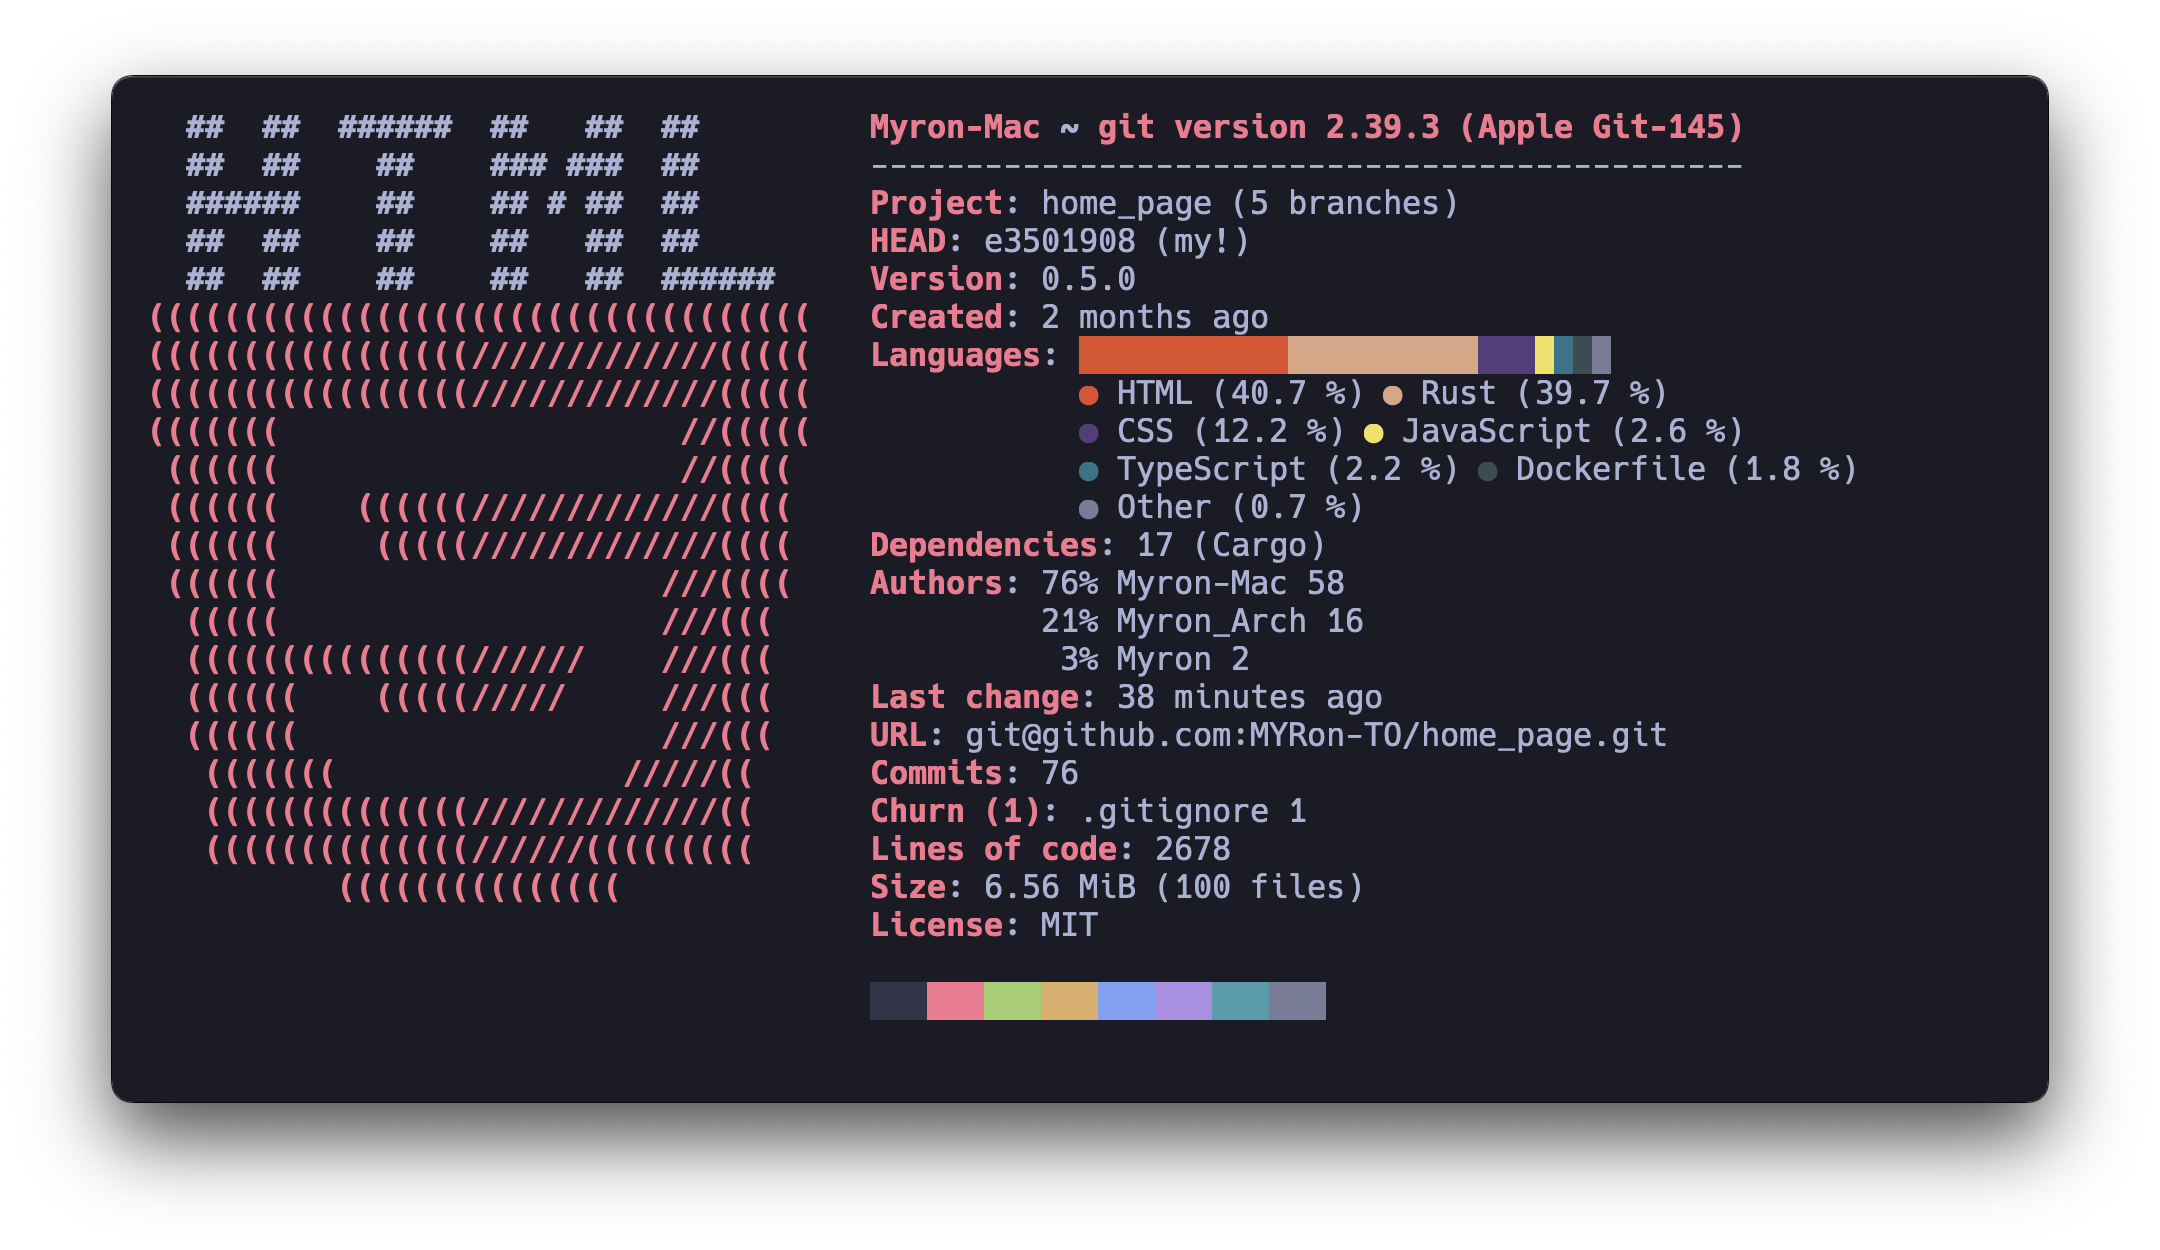
\includegraphics[width=1\textwidth]{pics/about_the_code.png}
	\caption{代码概述}
	\label{fig:about_the_code}
\end{figure}

Yuru 一个基于Axum的网站,使用Rust语言编写,
具有高并发、高性能、高可靠性的特点(大概)。
主要用于展示博客与个人简历。
只保留了最基本的功能,去除了一些不必要或没有意义的功能。
但添加了一些花里胡哨的东西。
图\ref{fig:about_the_code}是网站的代码概述。


\section{需求分析与功能说明}
本网站主要目的是展示博客与个人基本信息与联系方式。
具有高度个性化的特点。
使用者为网站所有者以及访问者。
因此需求分析主要从网站所有者的角度出发,
网站所有者需要的功能即需求。

经总结,本网站需要以下功能:
\begin{itemize}
	\item 渲染,展示博客
	\item 展示个人基本信息与联系方式
	\item 快速迅捷的分享功能
\end{itemize}

缺失的个人博客常见功能,
经过分析,大多为伪需求,
或使用者不需要的功能,
删去的功能有:
\begin{itemize}
	\item 点赞功能
  \item 编辑功能
\end{itemize}

点赞功能,属于伪需求,
点赞功能本身如同网站的浏览量一样,
可以由网站的所有者随意修改,
基本不具有参考价值。

编辑功能,使用者并不需要此功能,
访问者不需要编辑,
而现有的markdown编辑器,
编辑体验远远高于网站的编辑器,
从写作体验出发,
应使用现有的、成熟的编辑器。

暂未开发的功能有:
\begin{itemize}
  \item 网站的评论功能
  \item RSS订阅功能
\end{itemize}

未开发原因如下:

对于评论功能,
现有博客中,
评论系统大多依托于第三方服务,
自建的评论系统,
大多依托邮箱进行身份识别(登录),
无论使用还是管理都相对麻烦。
笔者希望依托于第三方服务,
如gitcomment,此服务依托于github,
使用github账号登录,
但使用前提是需要向github申请OAuth应用,
前提是网站需要有域名,
暂时没有域名,因此暂时无法使用此服务,
评论系统开发推迟。

对于RSS订阅功能,
由于时间原因,
笔者暂时没有详细了解RSS订阅功能,
因此推迟开发。

\section{功能分析与设计}

本网站具备以下功能:
\begin{itemize}
	\item 渲染,展示博客
	\item 分享功能
  \item 获取博客信息
\end{itemize}

\subsection{渲染博客}
渲染,展示博客,是本网站的主要功能,
博客使用markdown语法编写,
依赖于第三方库marked进行渲染。
利用AJAX技术,传输markdown文本,
并在前端渲染。
markdown文本路径以及基本信息,
如系列、标签等信息,存放于数据库中。
利用sqlx库,实现异步数据库操作。
关于博客的详细信息,
现有的手段通常为在文件开头添加元数据,
实现相对复杂,
本网站依赖于同目录下的json文件,
依赖于serde库,实现json文件的解析。

\subsection{分享博客}
分享功能,依托与浏览器原生的分享功能,
使用者可以快速分享网站的链接,
便于网站的传播。

\subsection{获取博客}
获取博客信息,
通过遍历博客文件夹,
读取博客的元数据,
整合进数据库中。

\section{界面设计与实现}
\subsection{界面设计}
本网站的界面设计,
主要使用了Material Design 2的设计规范,
相较于使用颜色来区分"高度"的Material Design 3,
Material Design 2使用阴影表示"高度",
个人认为更加灵动,
更适合表现"高度"和动态。
但由于阴影在深色主题难以表现,
Material Design 2的缺失了深色主题,
使得网站的包容性降低。

\subsection{界面实现}
实现上,使用了Material Design 2的组件库:
Material Design Lite,
该库简洁、轻量,
组件相对齐全,
可以方便的实现响应式布局,
方便快速开发。

\section{效果展示}
以下是网站的效果展示。

\begin{figure}[!htb]
	\centering
	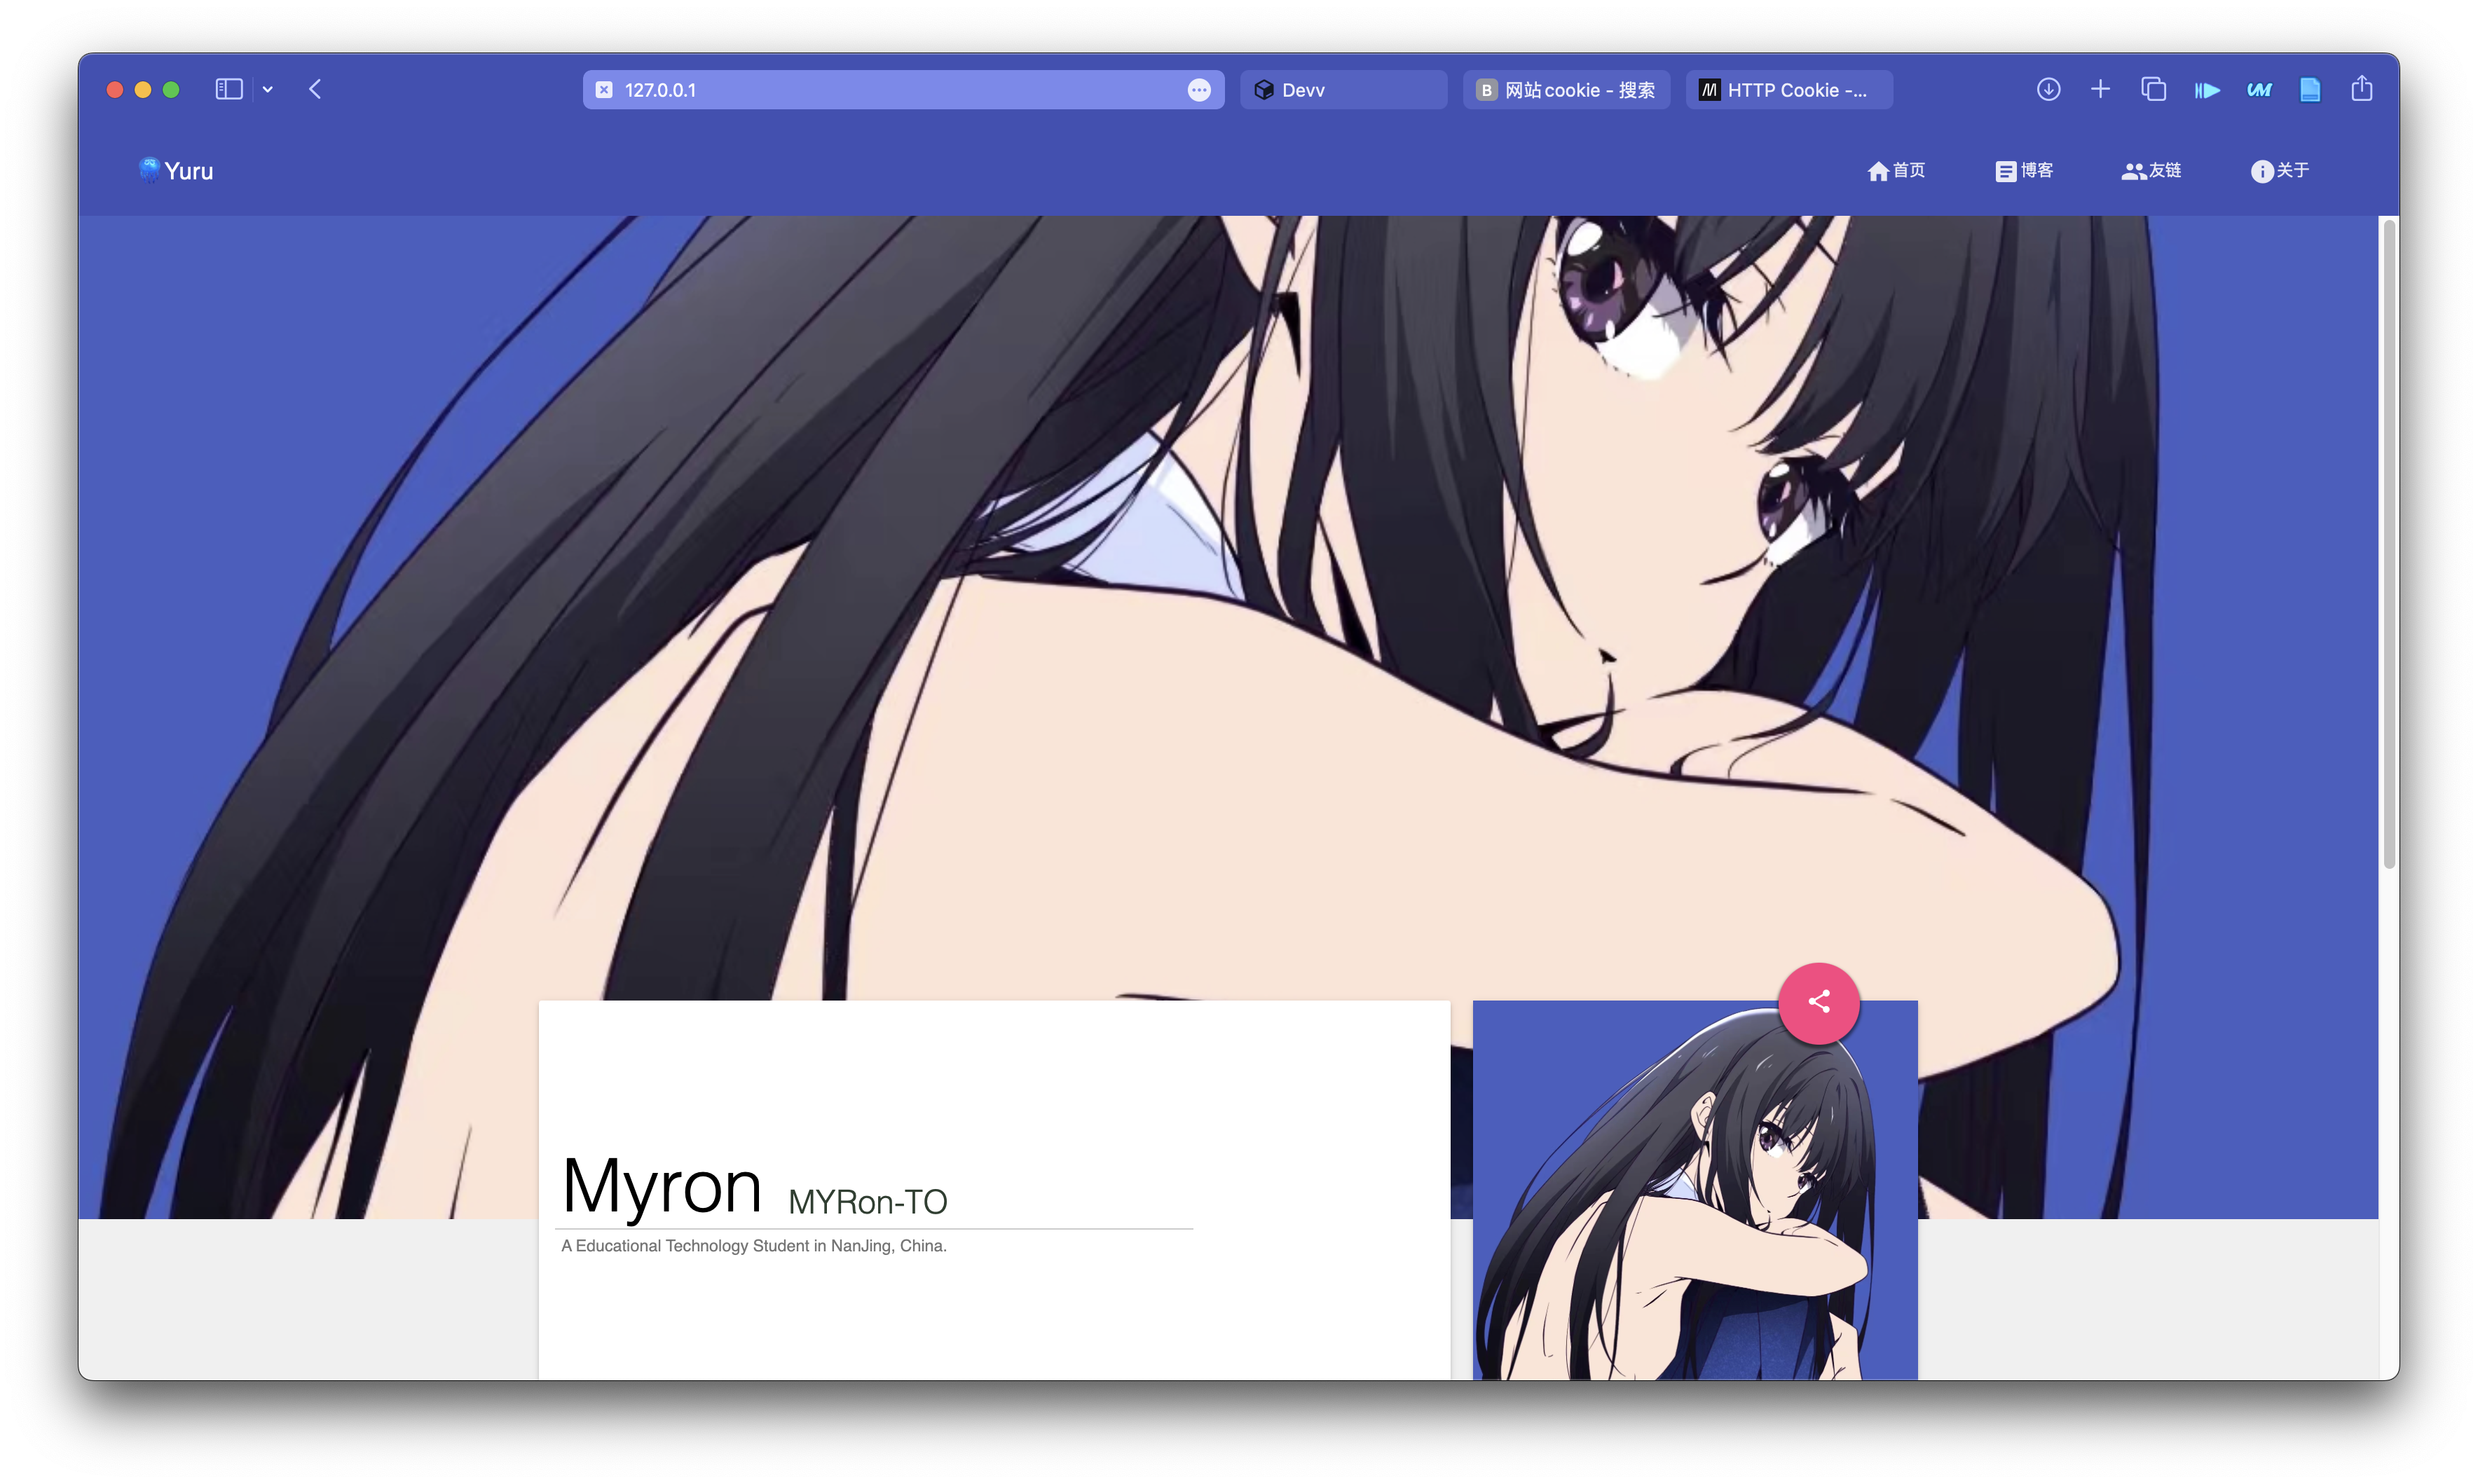
\includegraphics[width=1\textwidth]{pics/show_index.png}
	\caption{首页}
	\label{fig:show_index}
\end{figure}

\begin{figure}[!htb]
	\centering
	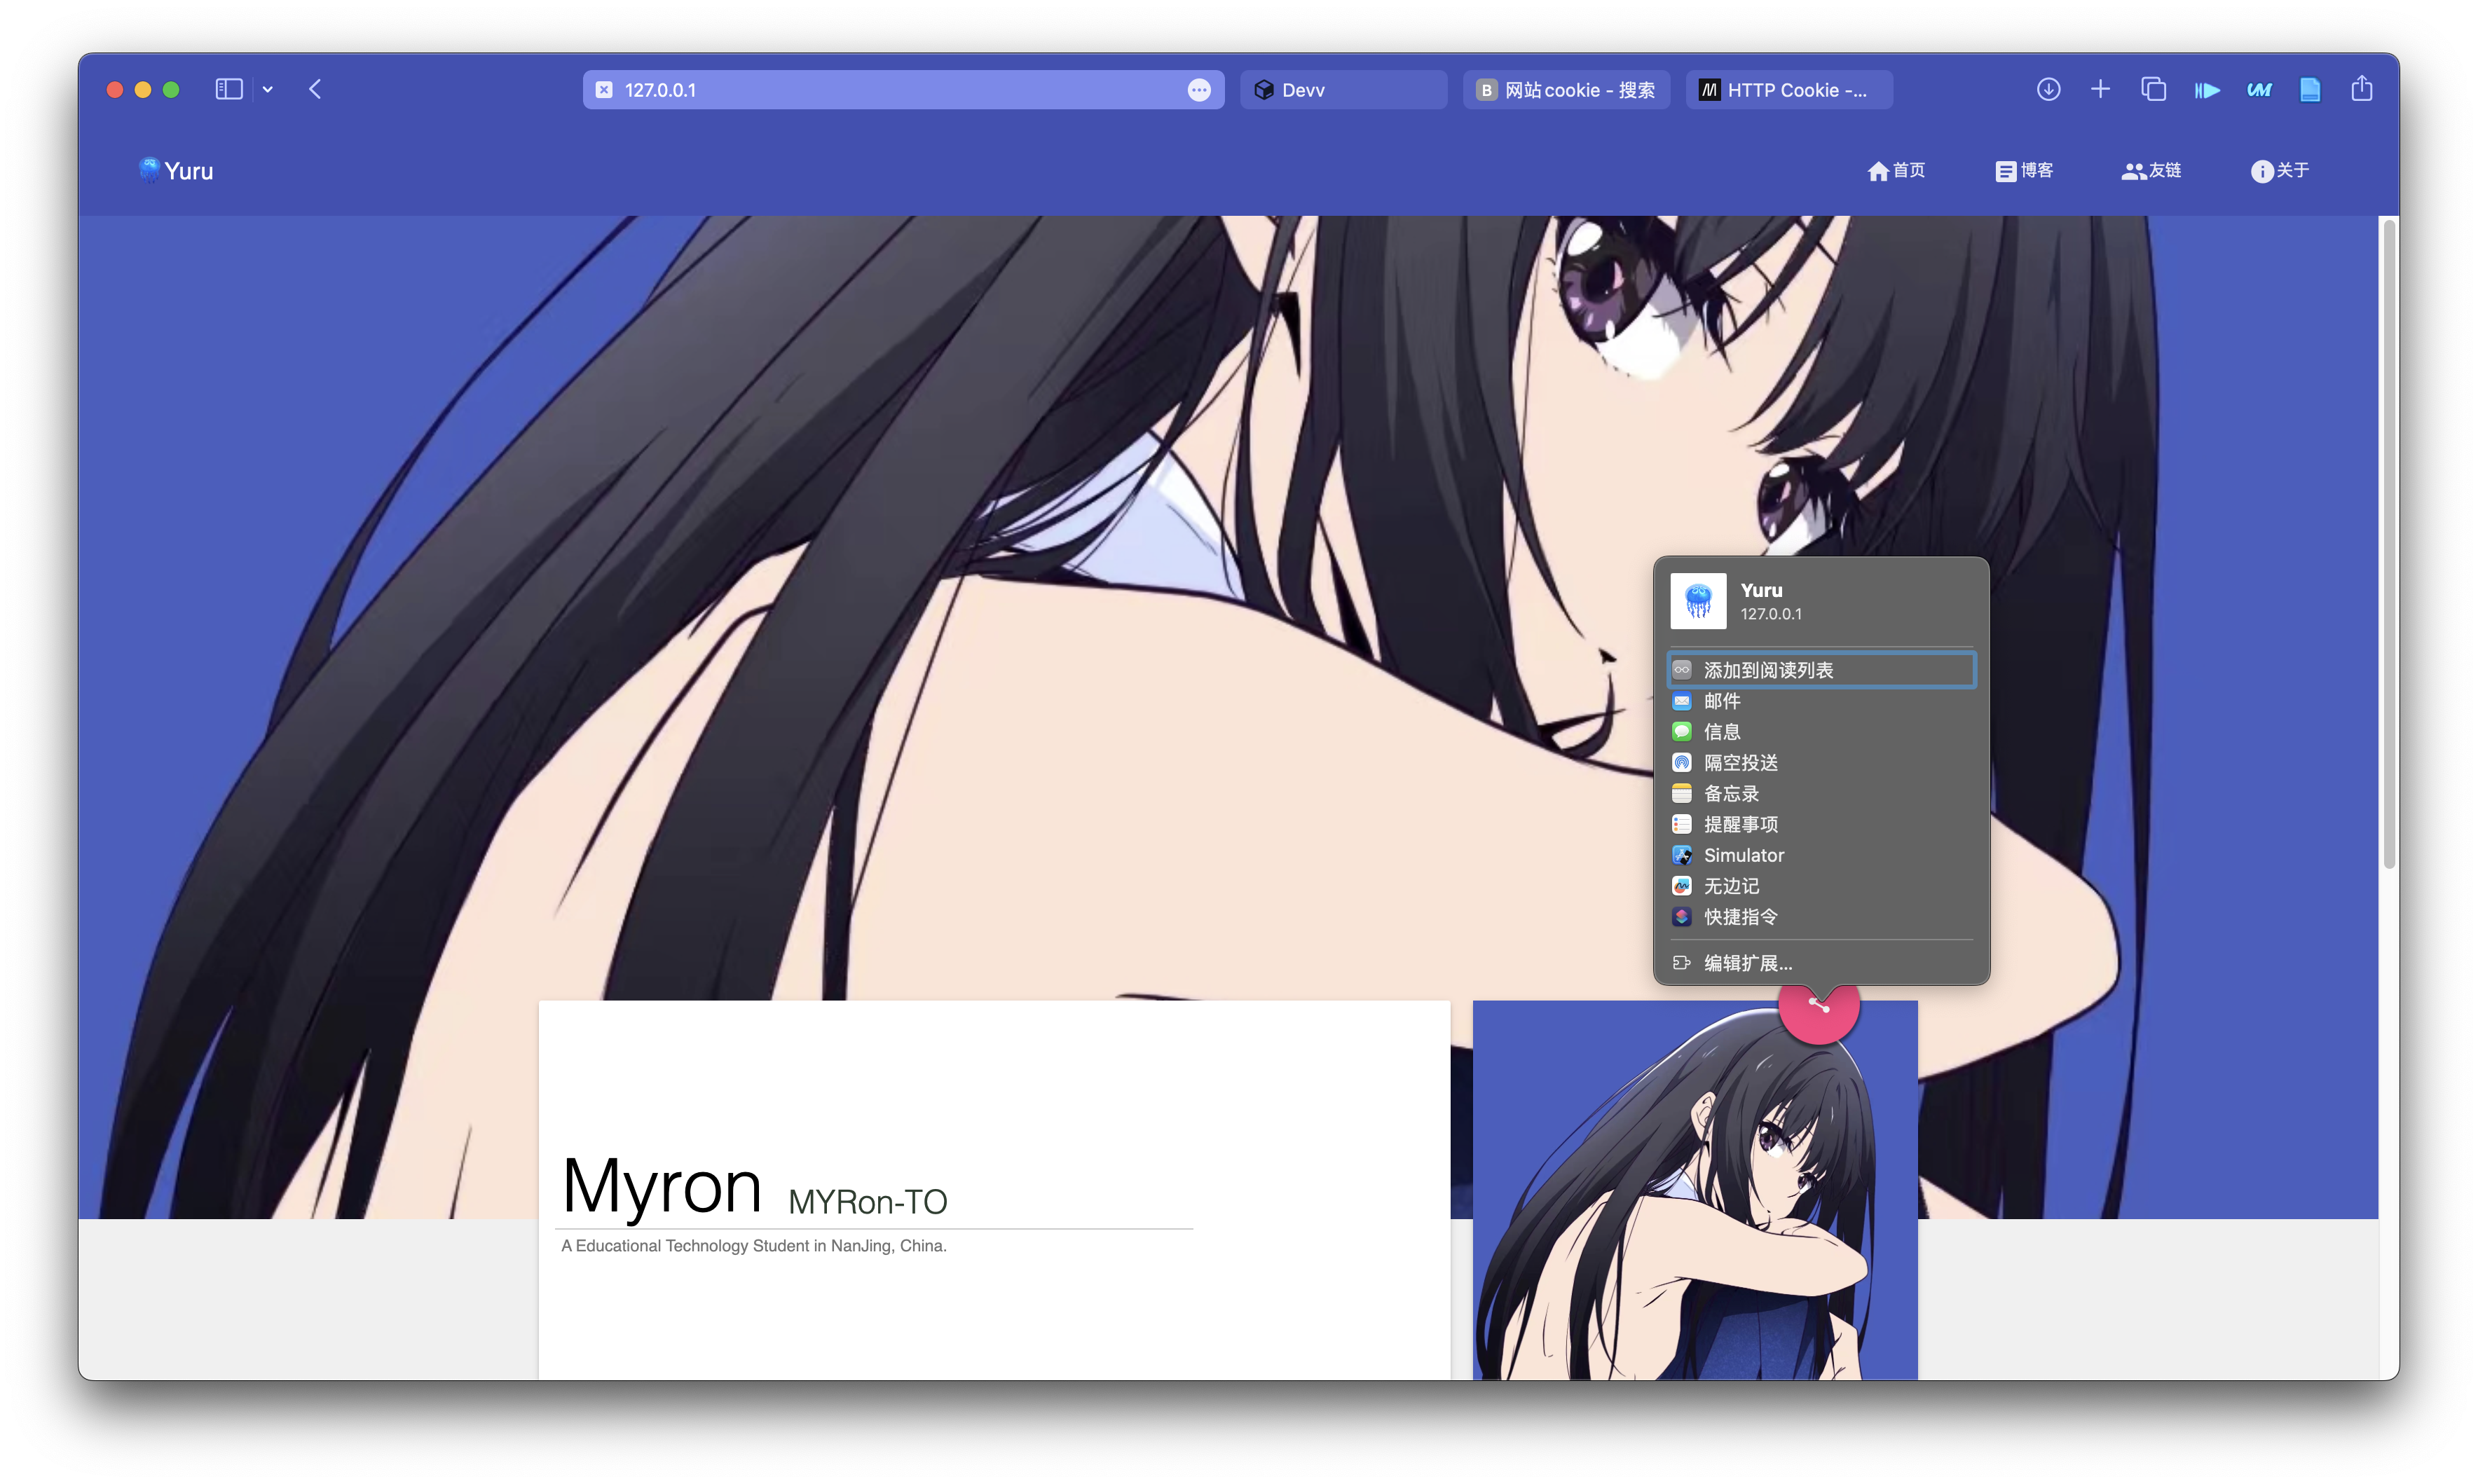
\includegraphics[width=1\textwidth]{pics/show_index_share.png}
	\caption{分享功能}
	\label{fig:show_index_share}
\end{figure}

\begin{figure}[!htb]
  \centering
  \includegraphics[width=1\textwidth]{pics/show_list.png}
  \caption{博客分类}
  \label{fig:show_list}
\end{figure}

\begin{figure}[!htb]
  \centering
  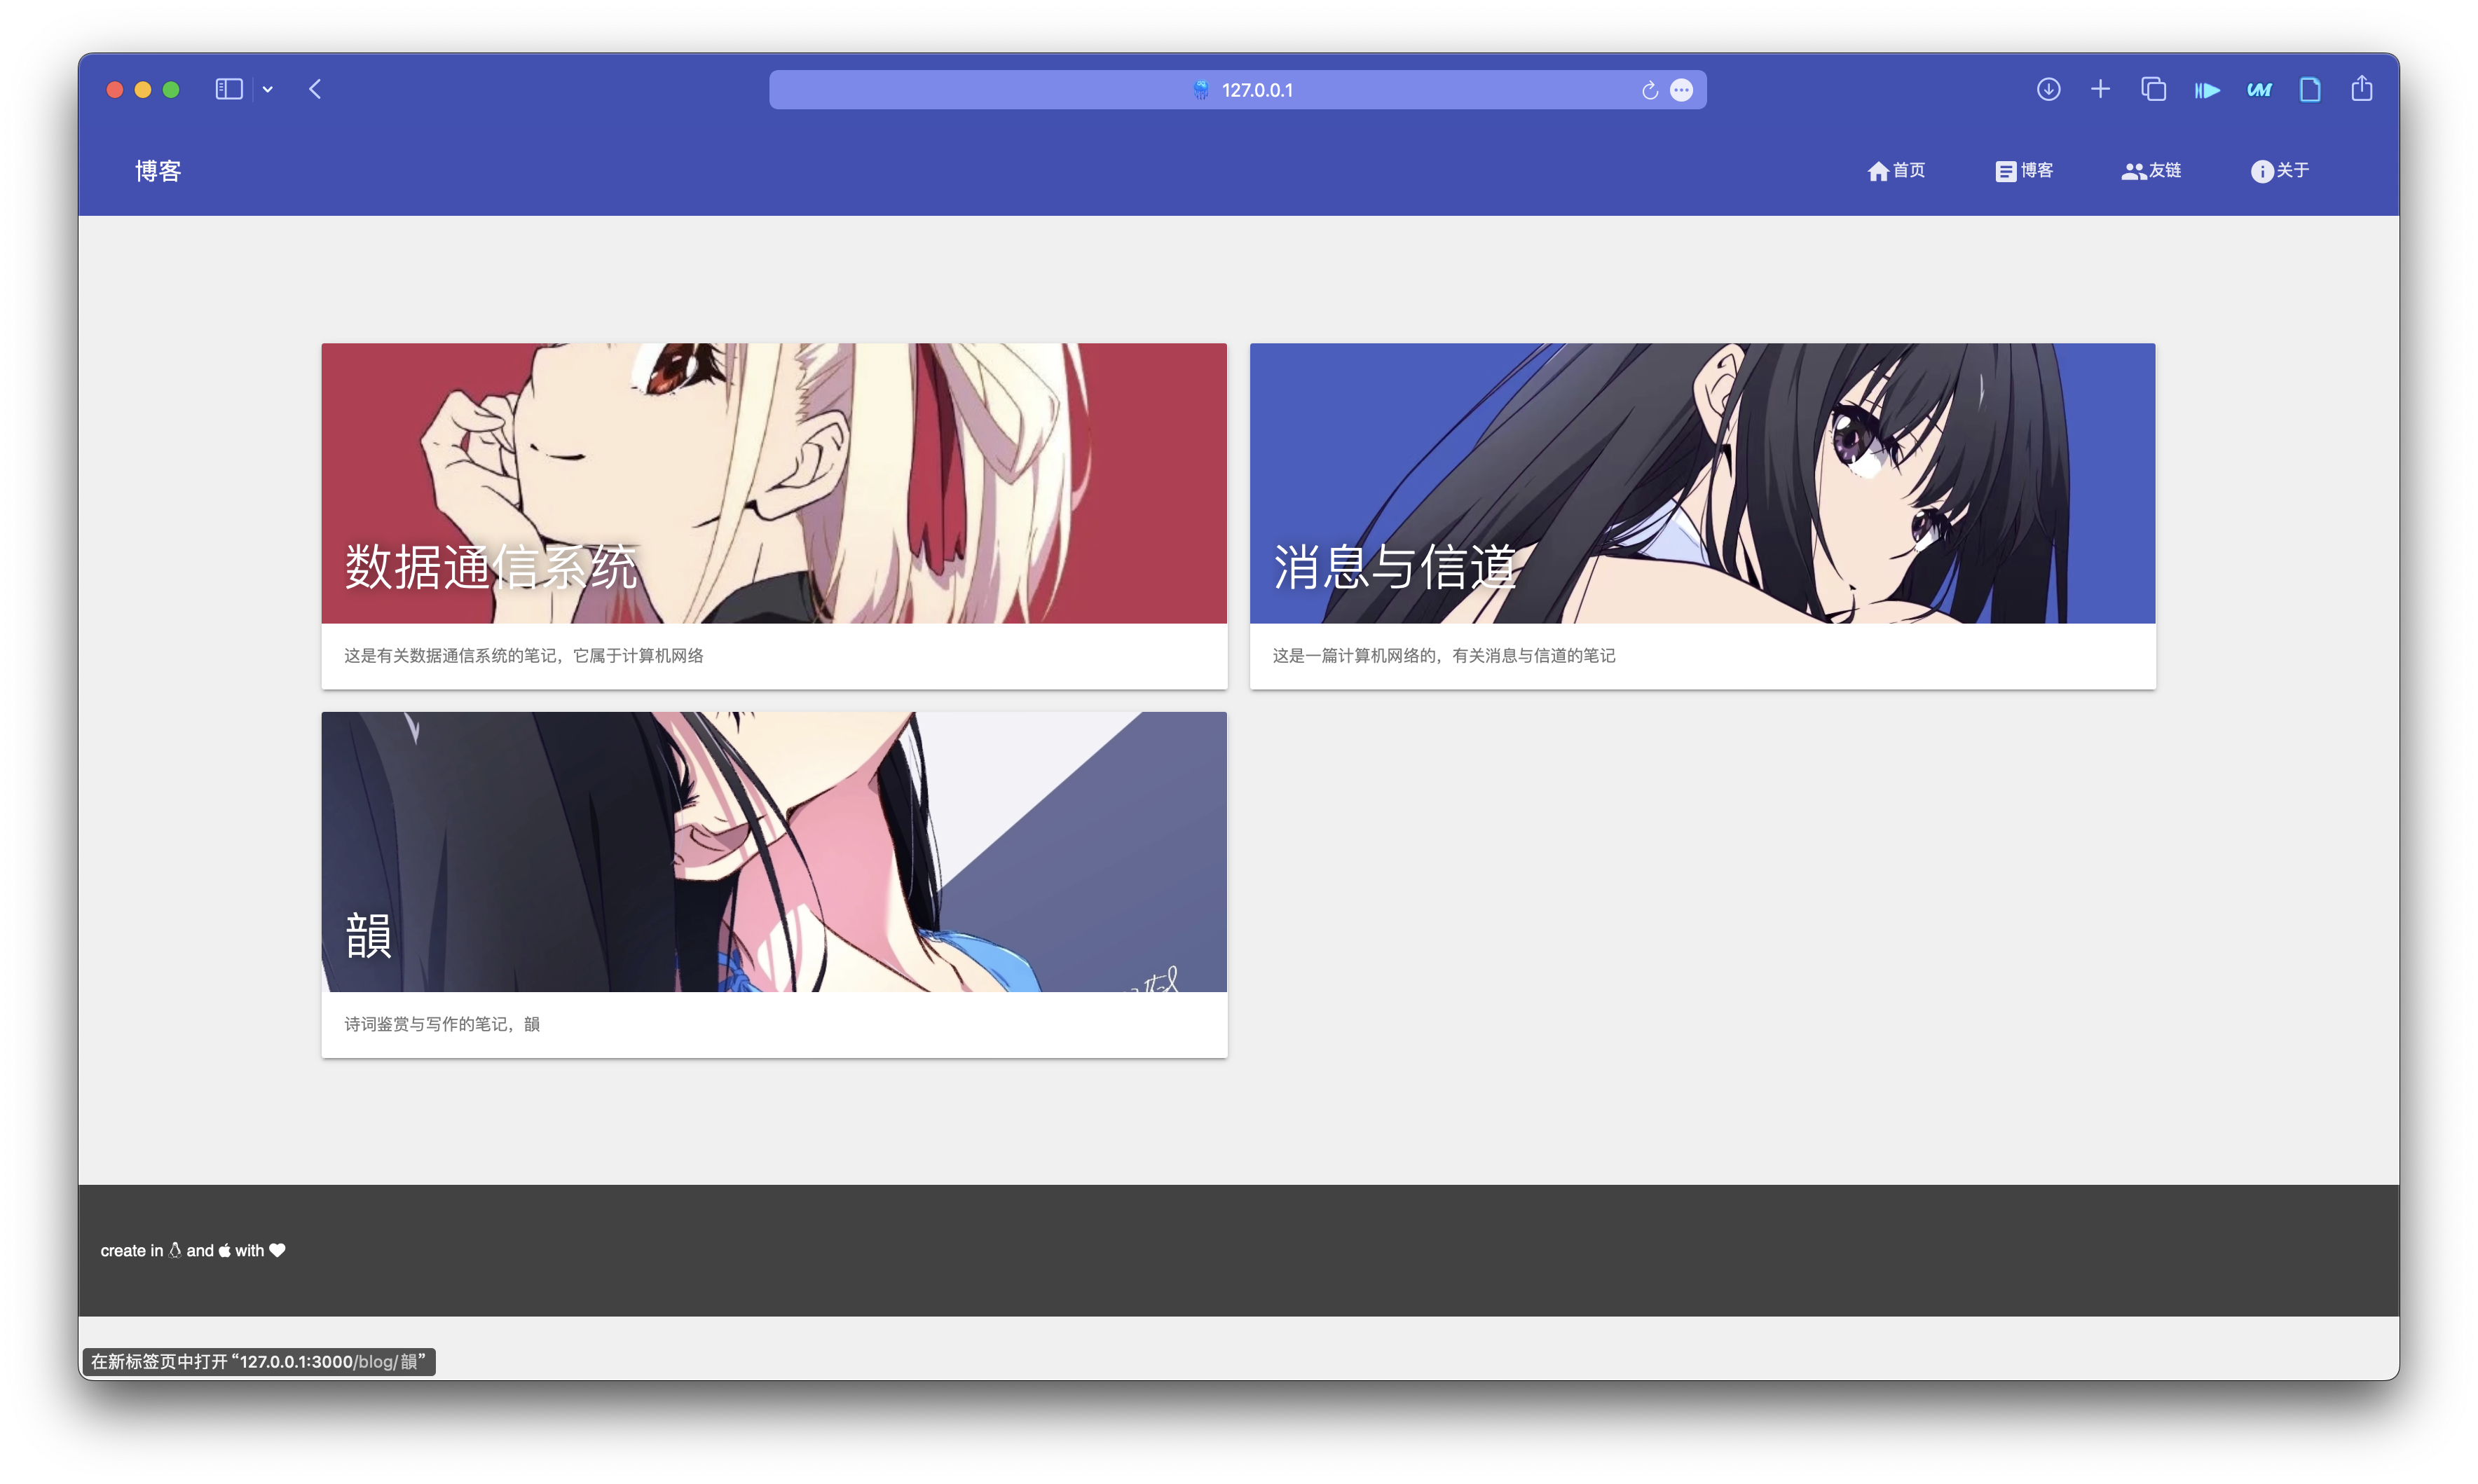
\includegraphics[width=1\textwidth]{pics/show_list_blog.png}
  \caption{博客列表}
  \label{fig:show_list_blog}
\end{figure}

\begin{figure}[!htb]
  \centering
  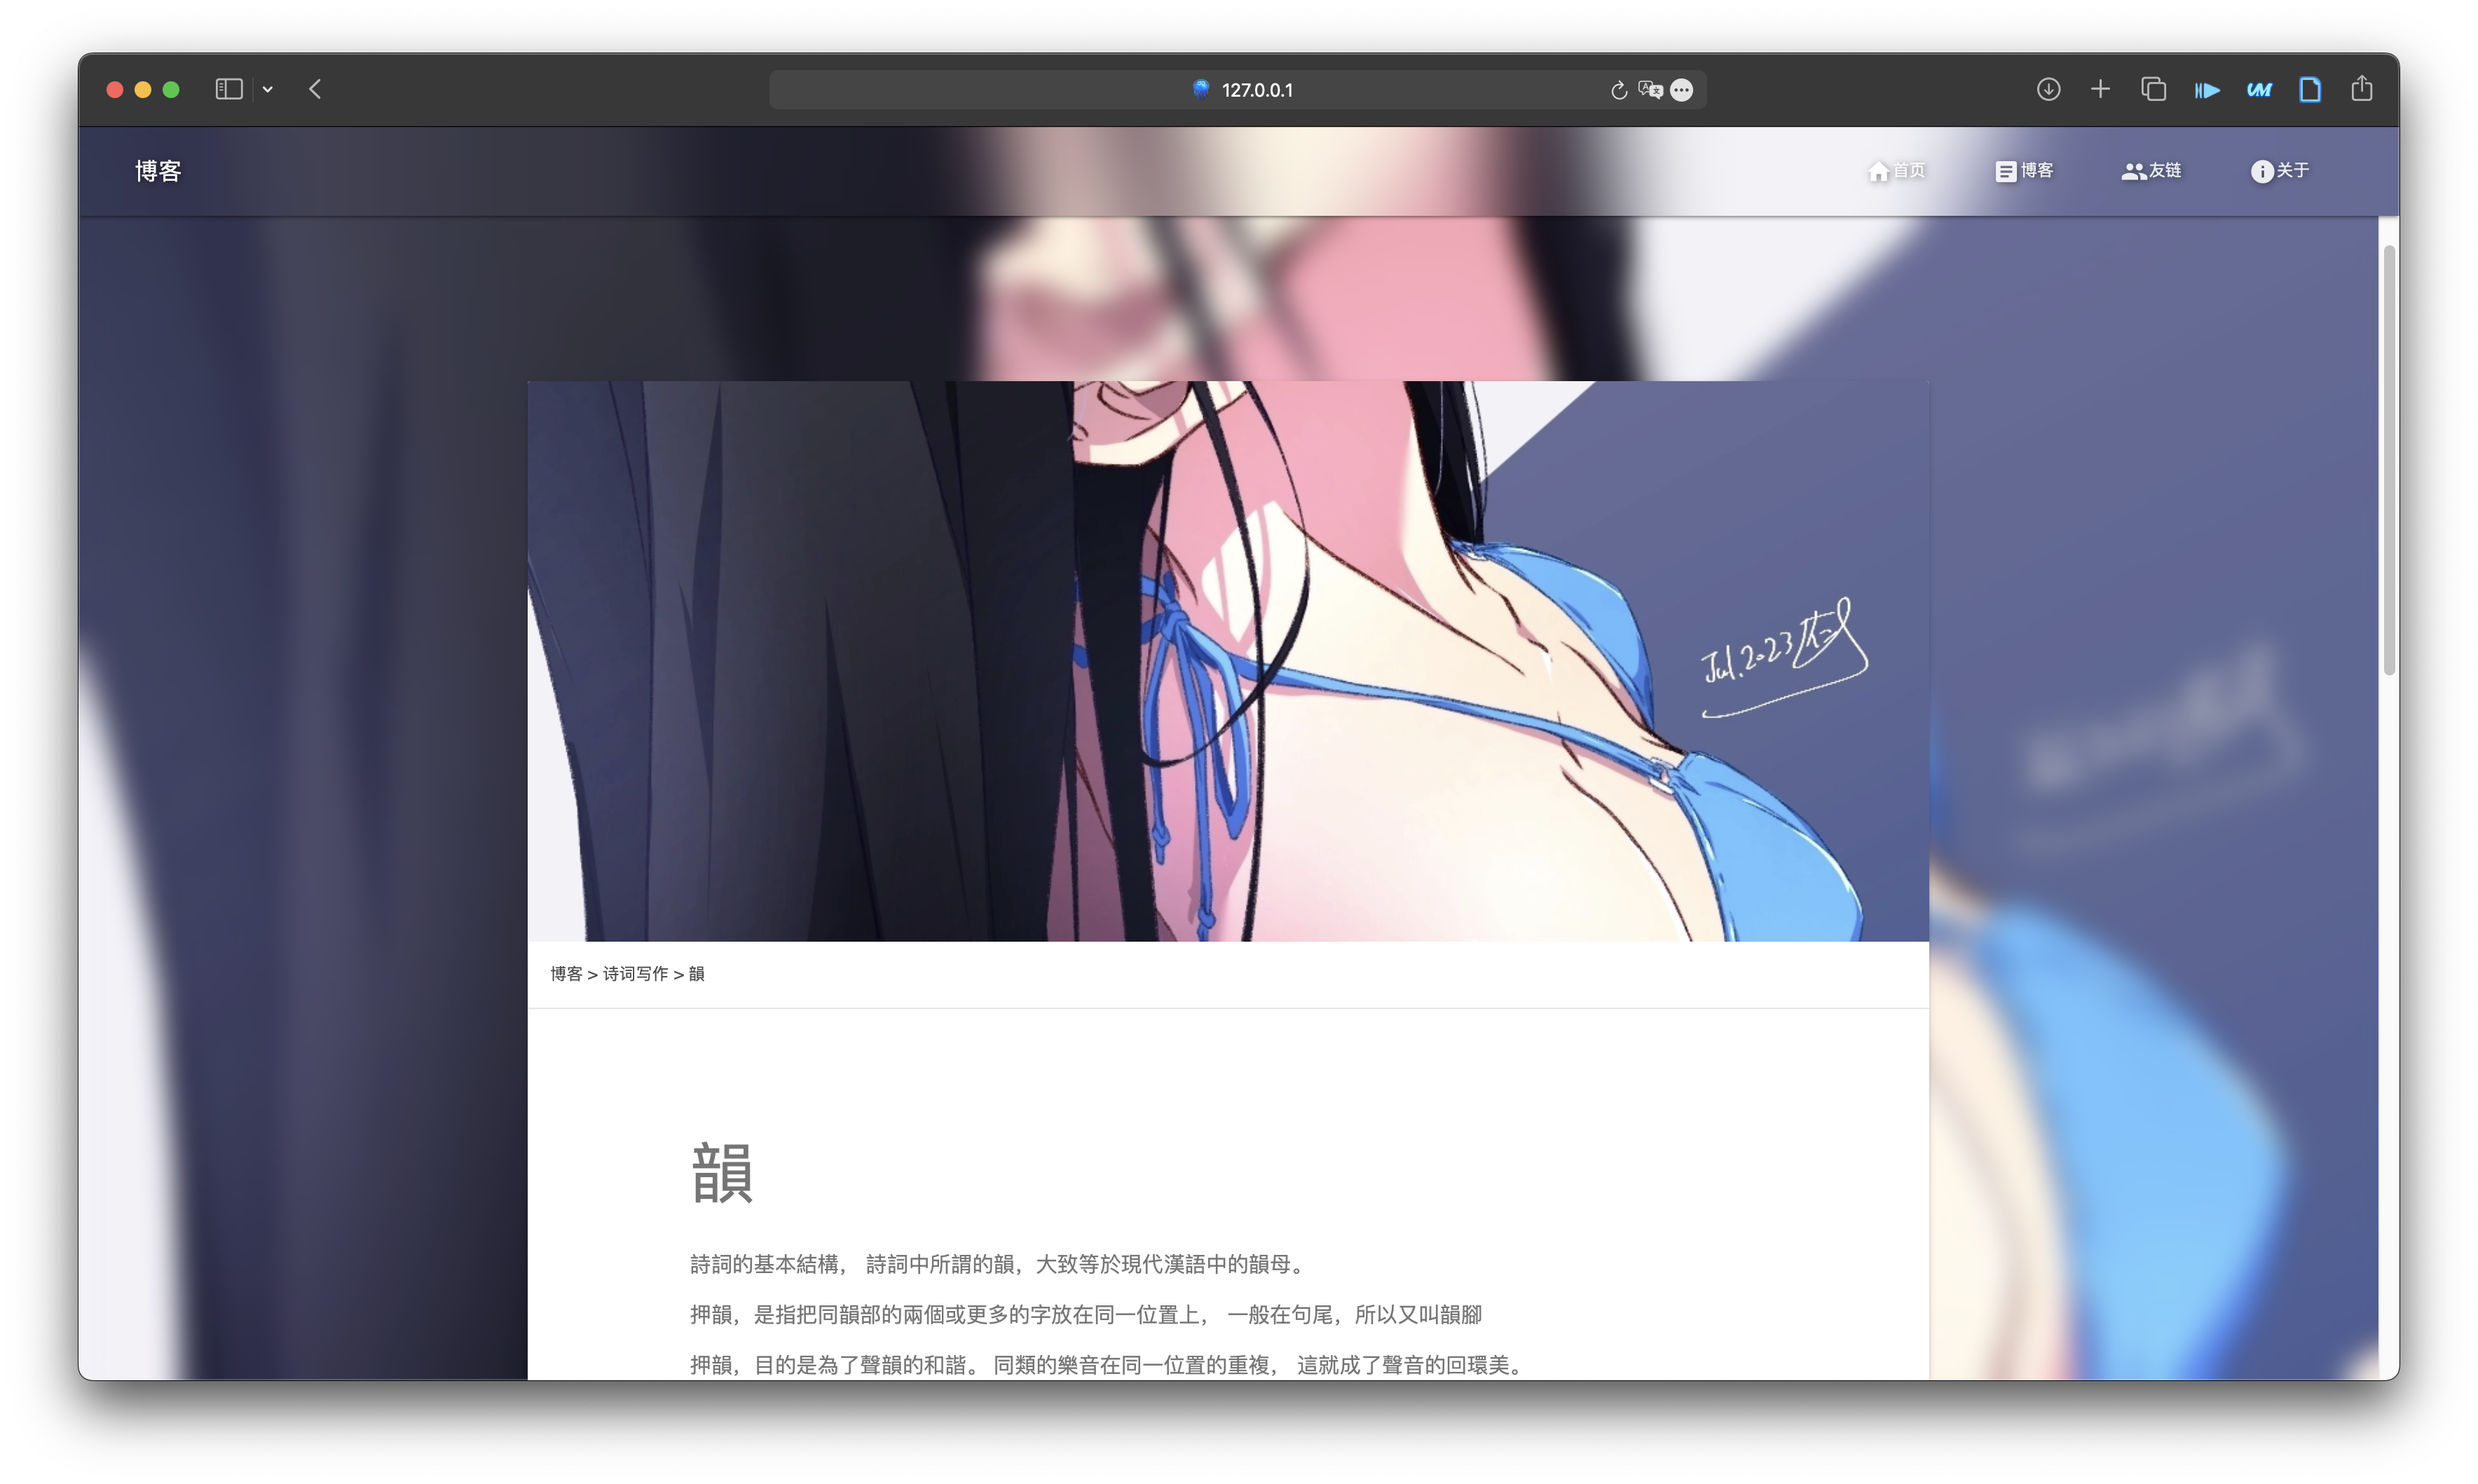
\includegraphics[width=1\textwidth]{pics/show_blog.png}
  \caption{博客内容1}
  \label{fig:show_blog_1}
\end{figure}

\begin{figure}[!htb]
  \centering
  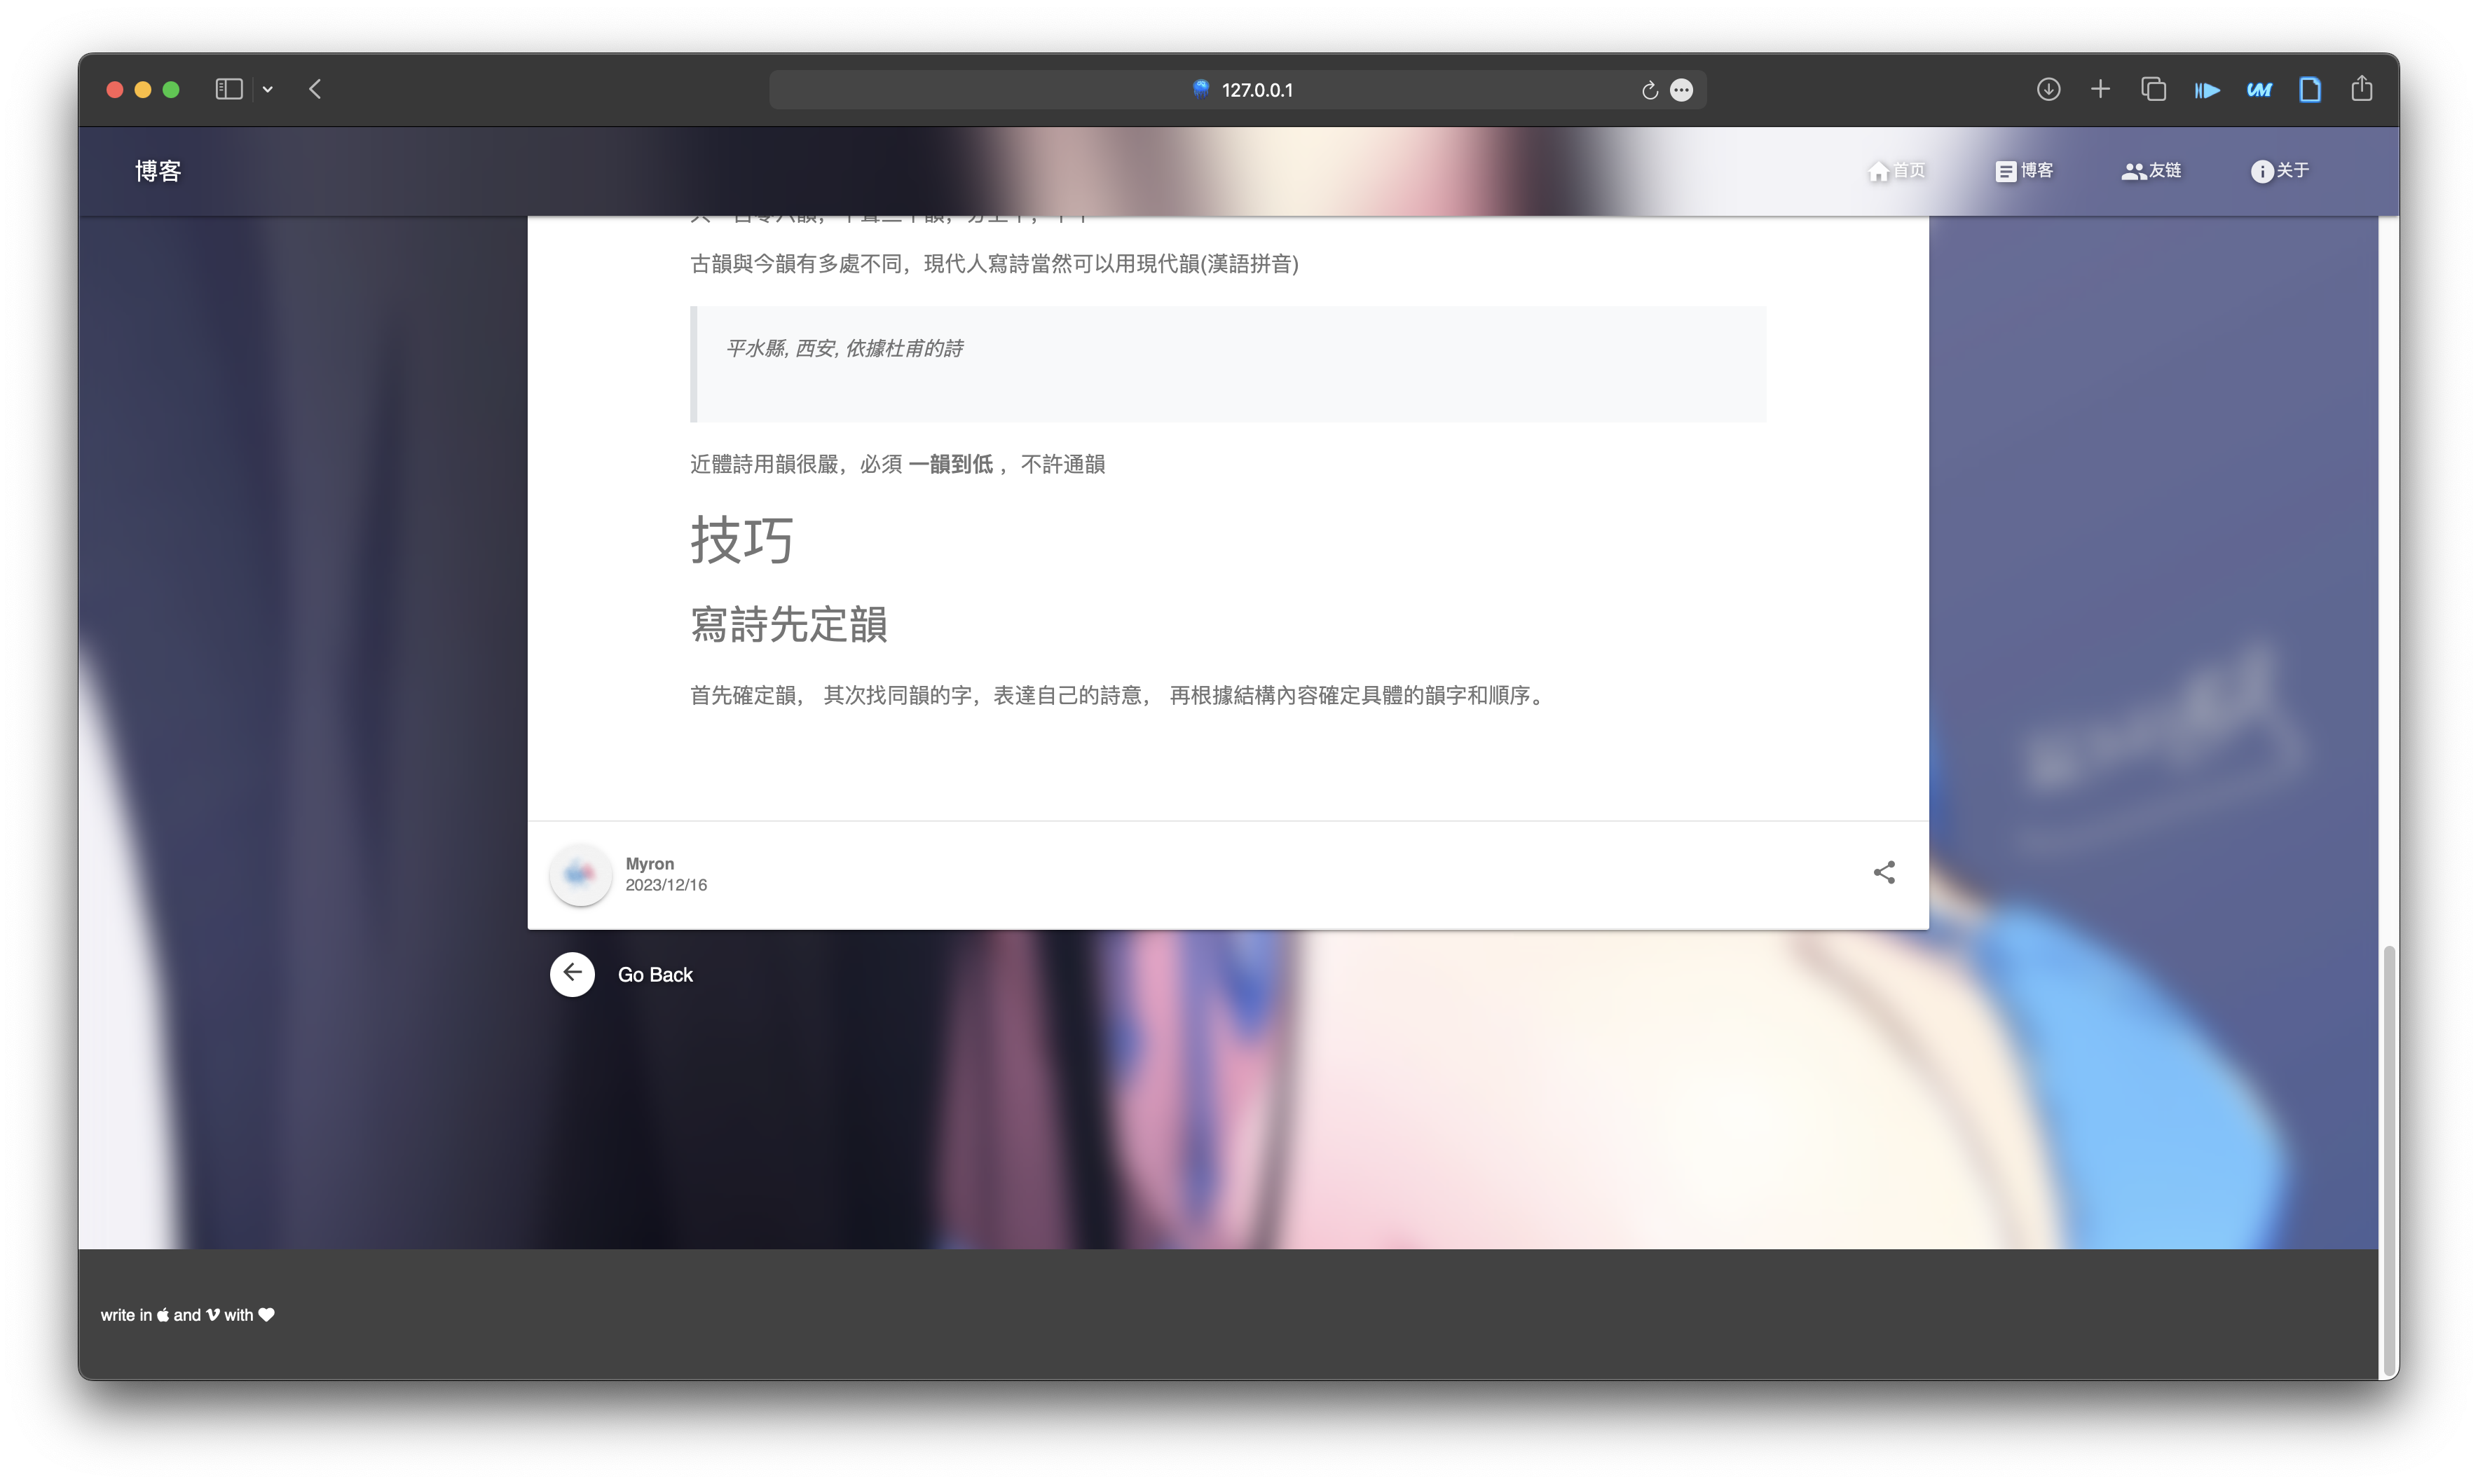
\includegraphics[width=1\textwidth]{pics/show_blog_2.png}
  \caption{博客内容2}
  \label{fig:show_blog_2}
\end{figure}

\begin{figure}[!htb]
  \centering
  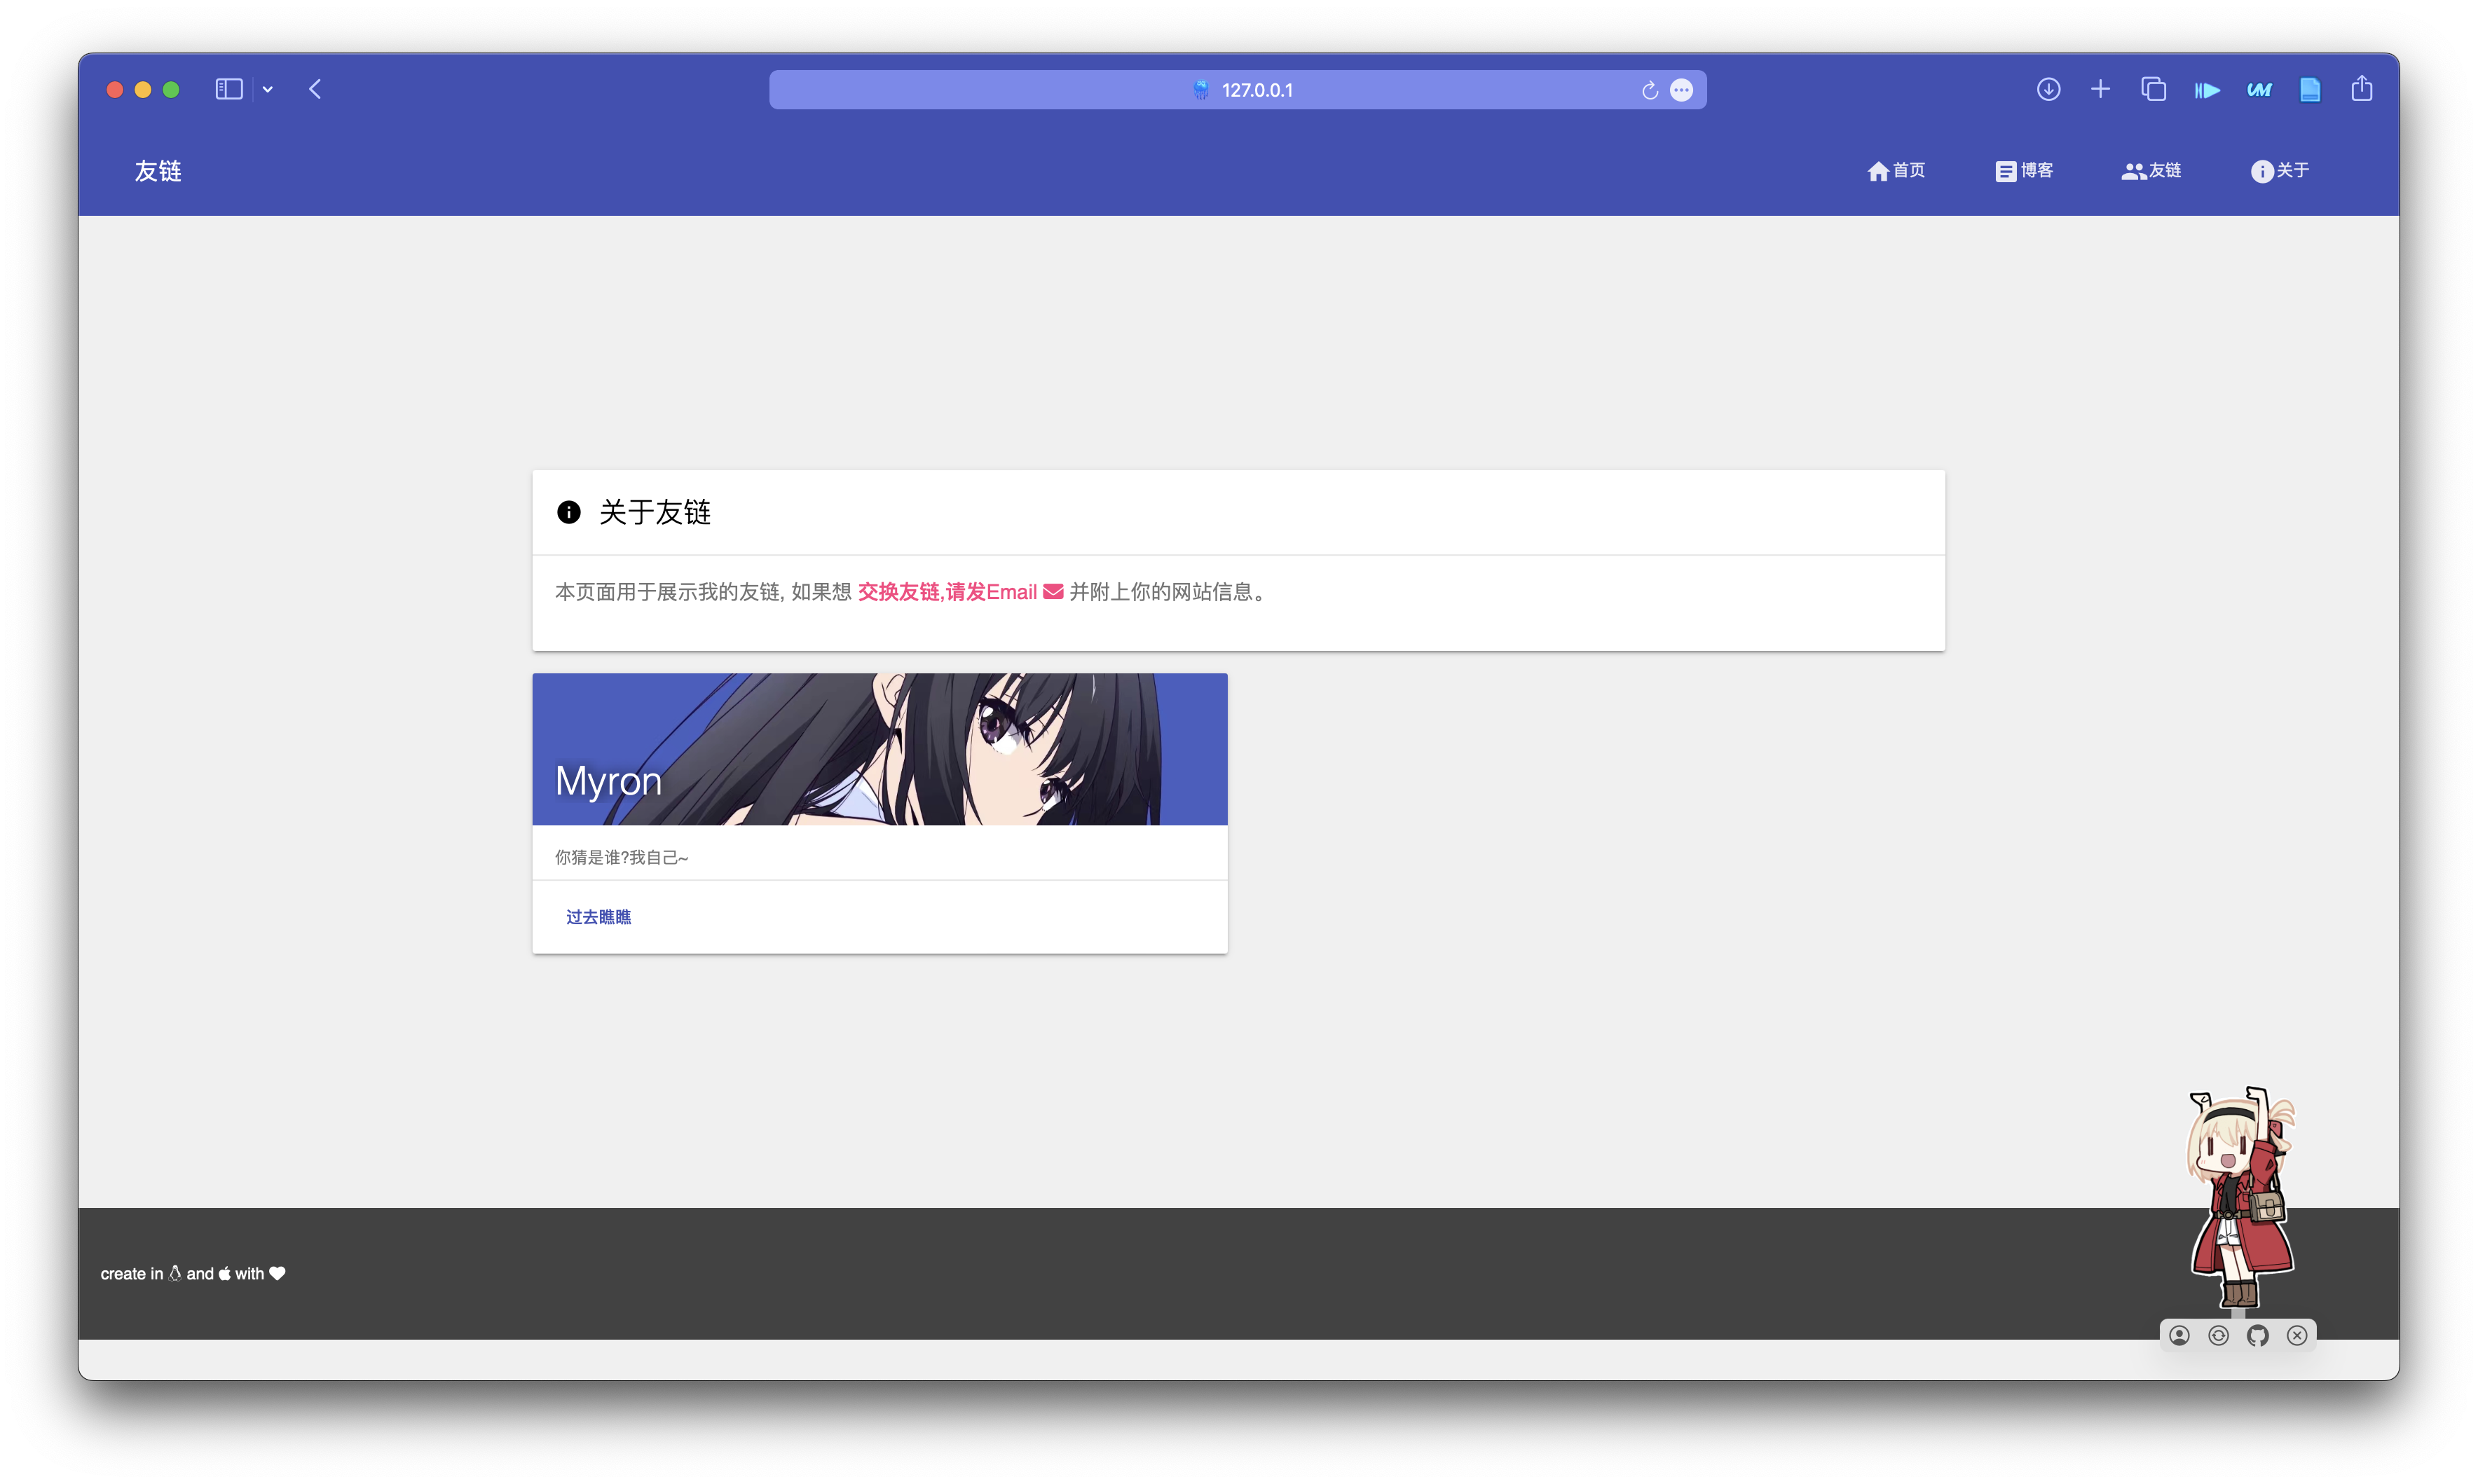
\includegraphics[width=1\textwidth]{pics/show_link.png}
  \caption{友链}
  \label{fig:show_link}
\end{figure}

\begin{figure}[!htb]
  \centering
  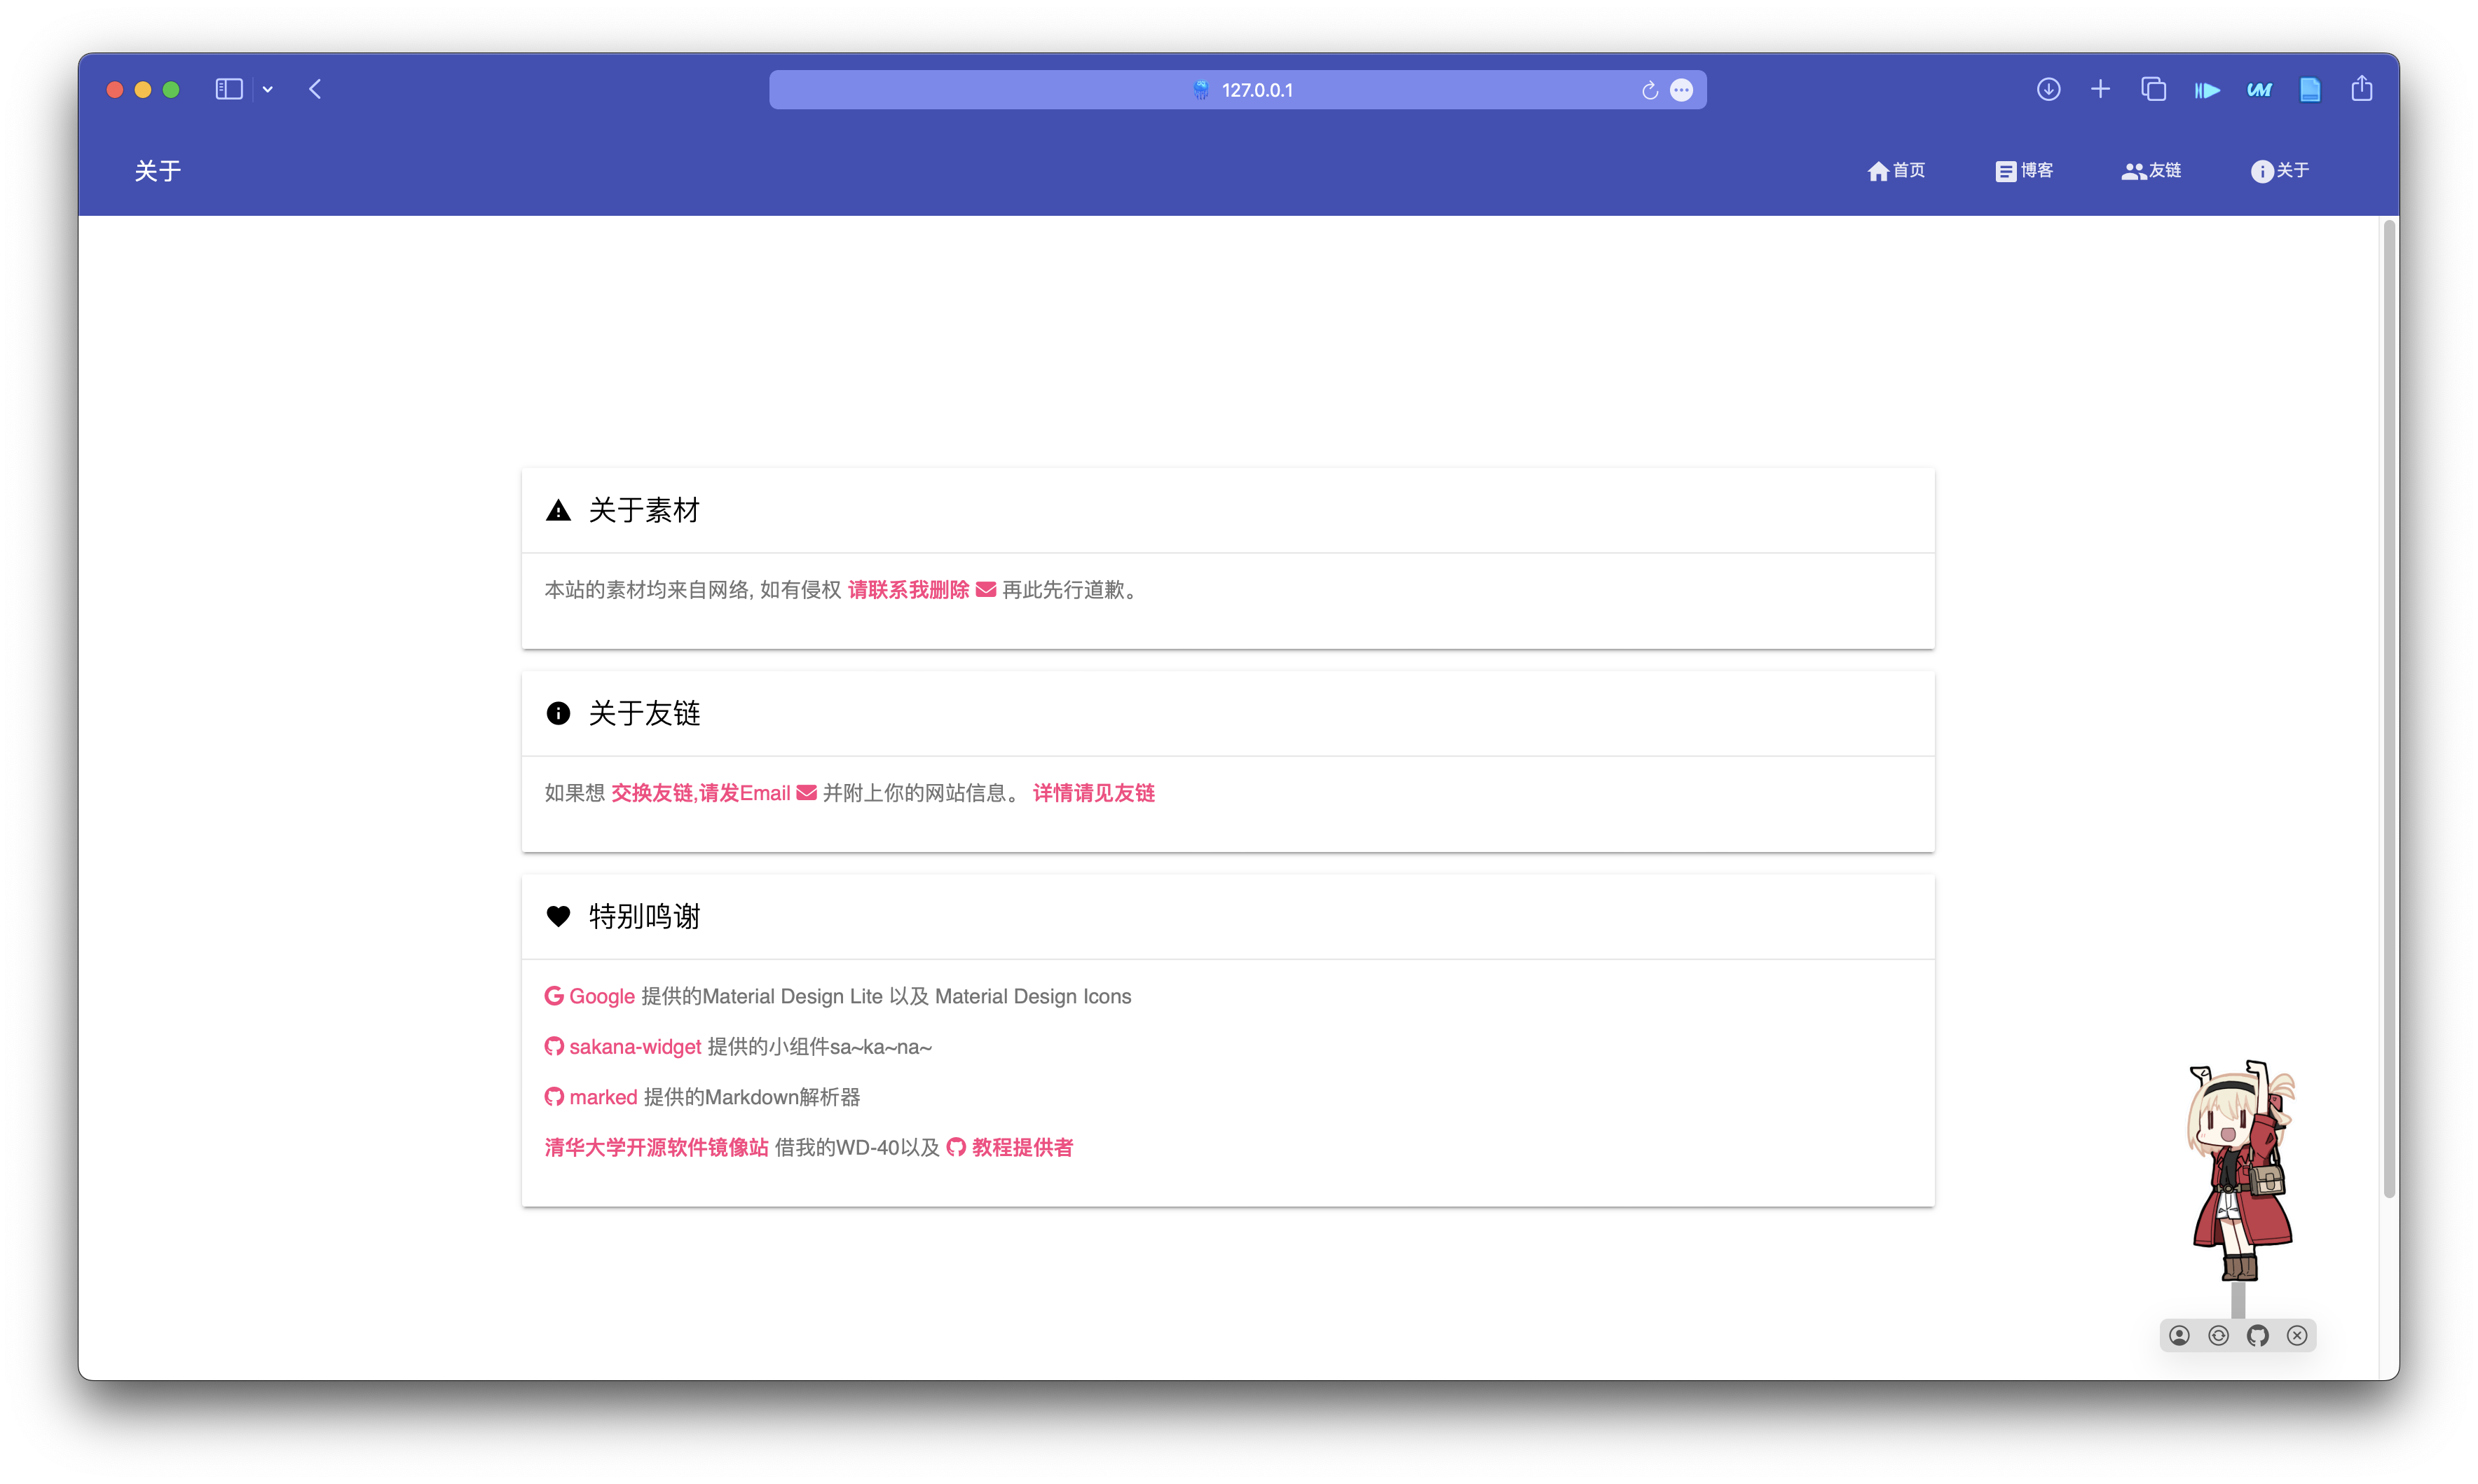
\includegraphics[width=1\textwidth]{pics/show_about.png}
  \caption{关于}
  \label{fig:show_about}
\end{figure}

图\ref{fig:show_index}是网站的首页。
图\ref{fig:show_index_share}是网站的分享功能。
此功能依赖于浏览器,部分浏览器(如firefox)可能无法使用此功能。

图\ref{fig:show_list}是网站的博客分类。
依照全部博客、系列、标签分类。
可以快速找到想要的博客。

图\ref{fig:show_list_blog}是网站的博客列表。

图\ref{fig:show_blog_1}是展示了具体的博客内容。

图\ref{fig:show_blog_2}是页面的底部。

图\ref{fig:show_link}是网站的友链。
暂时没有友链,所以写了一个指向本网站的友链。

图\ref{fig:show_about}是网站的关于页面。
展示了网站的一些信息。

\end{document}
